\section{Giao diện Web}

\subsection{Kiến trúc: trình duyệt, bridge và backend}
Trình duyệt không nói chuyện trực tiếp với server hay relay. Giữa chứng có một bridge viết bằng Python (\texttt{bridge.py}), phục vụ trang web qua HTTPS (mặc định cổng 8766) và làm cầu nối tới backend:
\begin{itemize}
    \item Chat và danh sách online: bridge duy trì kết nối TLS tới server core và chuyển sự kiện cho trình duyệt.
    \item File: tệp người dùng chọn được đưa vào vùng lưu tạm (staging) có giới hạn và gắn với đúng phiên, rồi một worker dùng \texttt{FileClient} gửi qua từng UDP relay. Phía nhận cũng đi theo đường ngược lại, và người dùng tải file về từ bridge.
\end{itemize}

Khóa phiên và ticket chỉ nằm ở phía bridge. Chúng không bao giờ được chuyển cho JavaScript trong trình duyệt. Phần giao diện (renderer và reducer) được tách khỏi lớp kết nối với backend, đúng yêu cầu của đề về việc tách sử lý mạng, xử lý dữ liệu và giao diện.

\subsection{Luồng sử dụng}
Người dùng mở \texttt{https://127.0.0.1:8766/}, đăng nhập bằng tài khoản đã có (giao diện chỉ có chức năng đăng nhập, tài khoản thử được tạo qua \texttt{REGISTER} trên kênh TLS), rồi thực hiện các thao tác sau:
\begin{enumerate}
    \item Danh sách người dùng: Thanh bên liệt kê các cuộc trò chuyện và mục Người đang hoạt đồng, chỉ lọc những người đang online. NGười dùng tìm người theo tên bằng nút kính lúp, tìm không phân biệt hoa thường và dấu.
    \item Chat chung và chat riêng. Người dùng chọn “Kênh chung” (trò chuyện với mọi người đang kết nối) hoặc một người cụ thể. Tiêu đề luôn ghi loại chat và người nhận để tránh gửi nhầm. Bản nháp và lịch sử được giữ riêng cho từng cuộc trò chuyện.
    \item Gửi và nhận file. Người gửi chọn file trong cuộc chat riêng. Người nhận thấy thẻ file và chọn Chấp nhận hoặc Từ chối. Thẻ hiển thị trạng thái và thanh tiến trình trong lúc truyền, sau đó người nhận tải file về và đối chiếu SHA-256. Chat vẫn dùng được trong lúc file đang truyền.
    \item Ngắt và kết nối lại. Khi người dùng ngắt kết nối, người còn lại thấy họ offline nhưng vẫn giữ nguyên cuộc trò chuyện và bản nháp; đăng nhập lại là dùng được ngay.
\end{enumerate}

\noindent
\begin{minipage}[t]{0.48\textwidth}
    \centering
    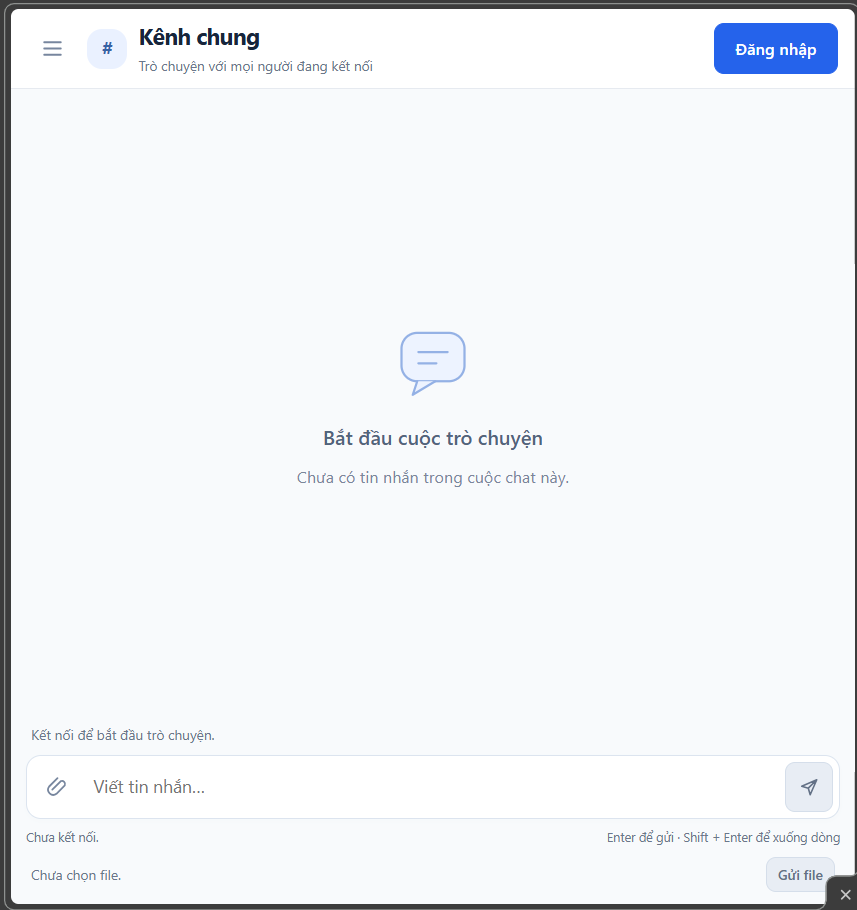
\includegraphics[width=\textwidth]{Assets/login.png}
\end{minipage}
\hfill
\begin{minipage}[t]{0.48\textwidth}
    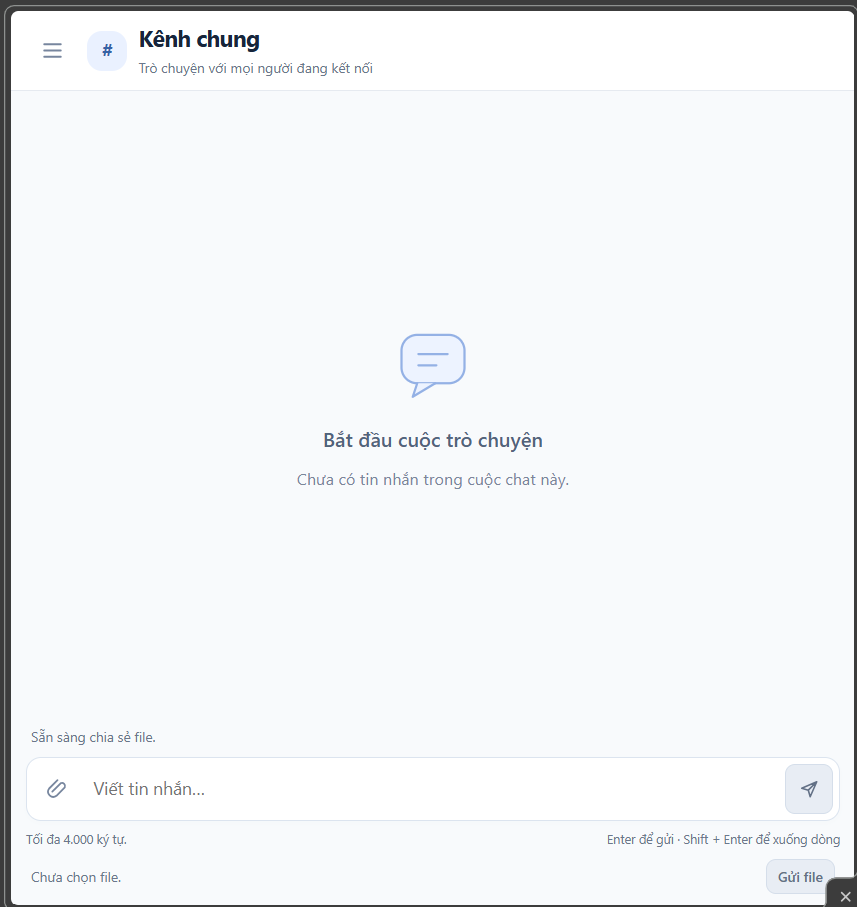
\includegraphics[width=\textwidth]{Assets/lobby.png}
\end{minipage}
\begin{center}
    \captionof{figure}{Giao diện màn hình đăng nhập và màn hình chính}
\end{center}

\noindent
\begin{minipage}[t]{0.48\textwidth}
    \centering
    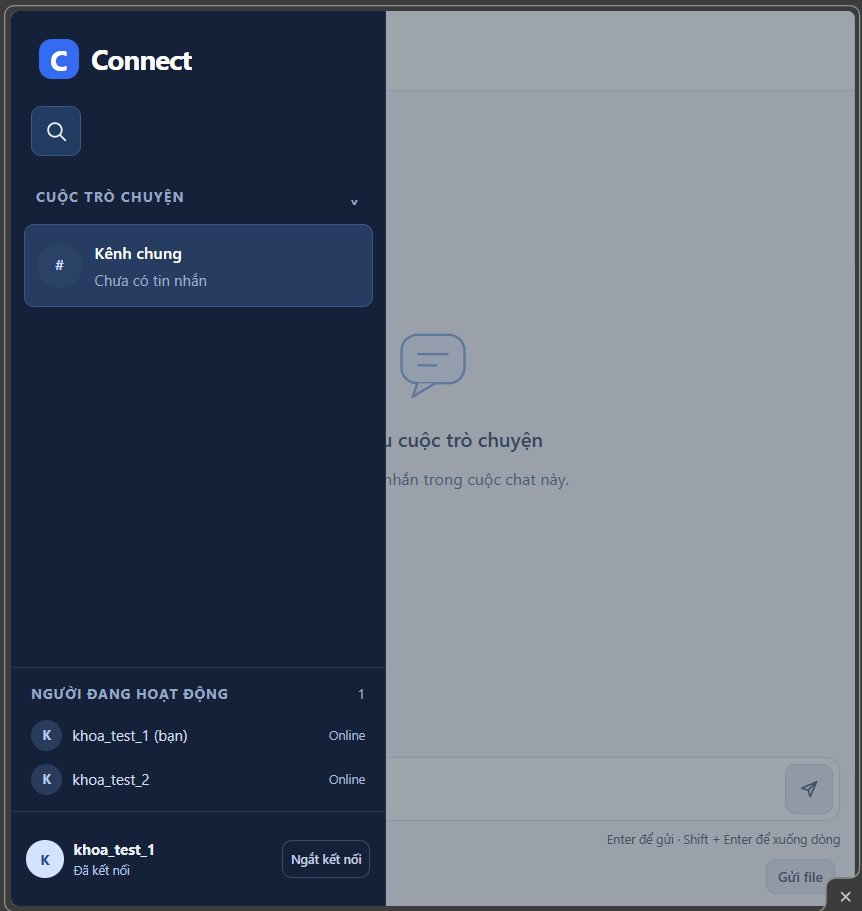
\includegraphics[width=\textwidth]{Assets/sidebar.png}
\end{minipage}
\hfill
\begin{minipage}[t]{0.48\textwidth}
    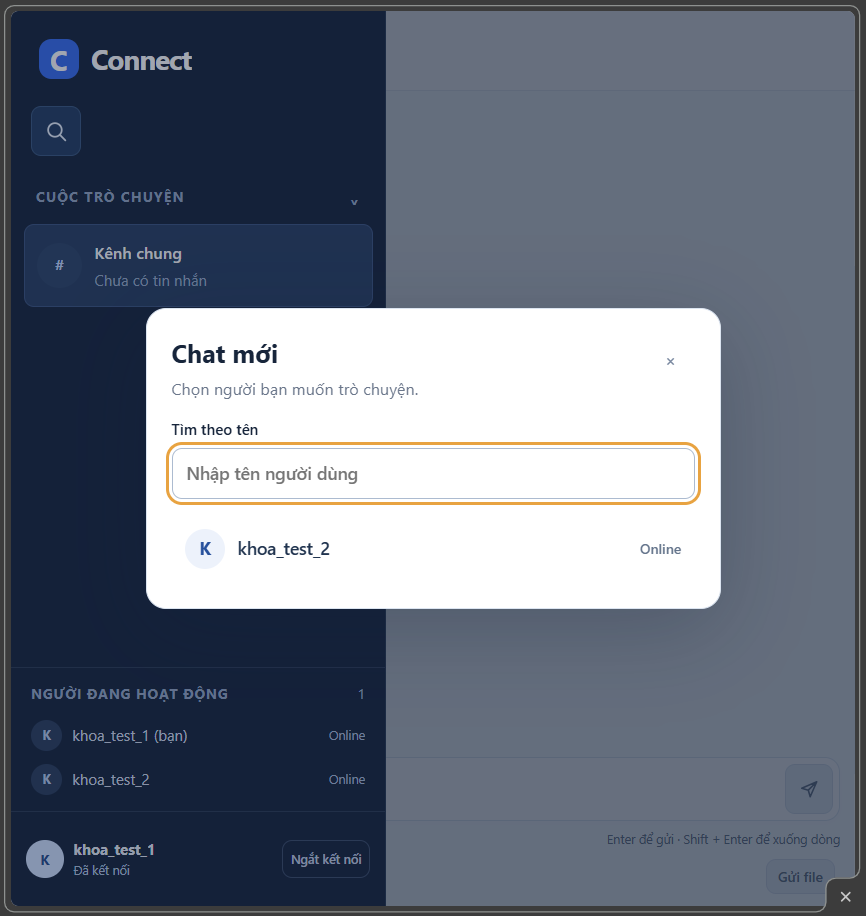
\includegraphics[width=\textwidth]{Assets/search_panel.png}
\end{minipage}
\begin{center}
    \captionof{figure}{Thanh bên và bảng tìm kiếm}
\end{center}

\noindent
\begin{minipage}[t]{0.48\textwidth}
    \centering
    
\includegraphics[width=\textwidth]{Assets/login_panel.jpg}
\end{minipage}
\hfill
\begin{minipage}[t]{0.48\textwidth}
    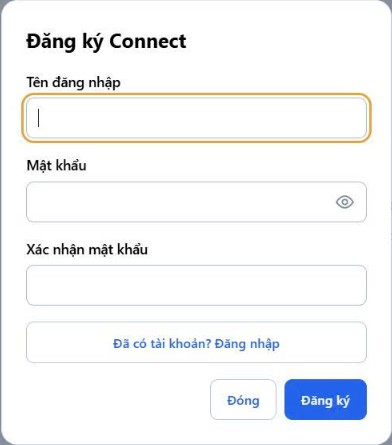
\includegraphics[width=\textwidth]{Assets/register_panel.jpg}
\end{minipage}
\begin{center}
    \captionof{figure}{Khung đăng nhập và đăng ký}
\end{center}

\begin{figure}[H]
    \centering
    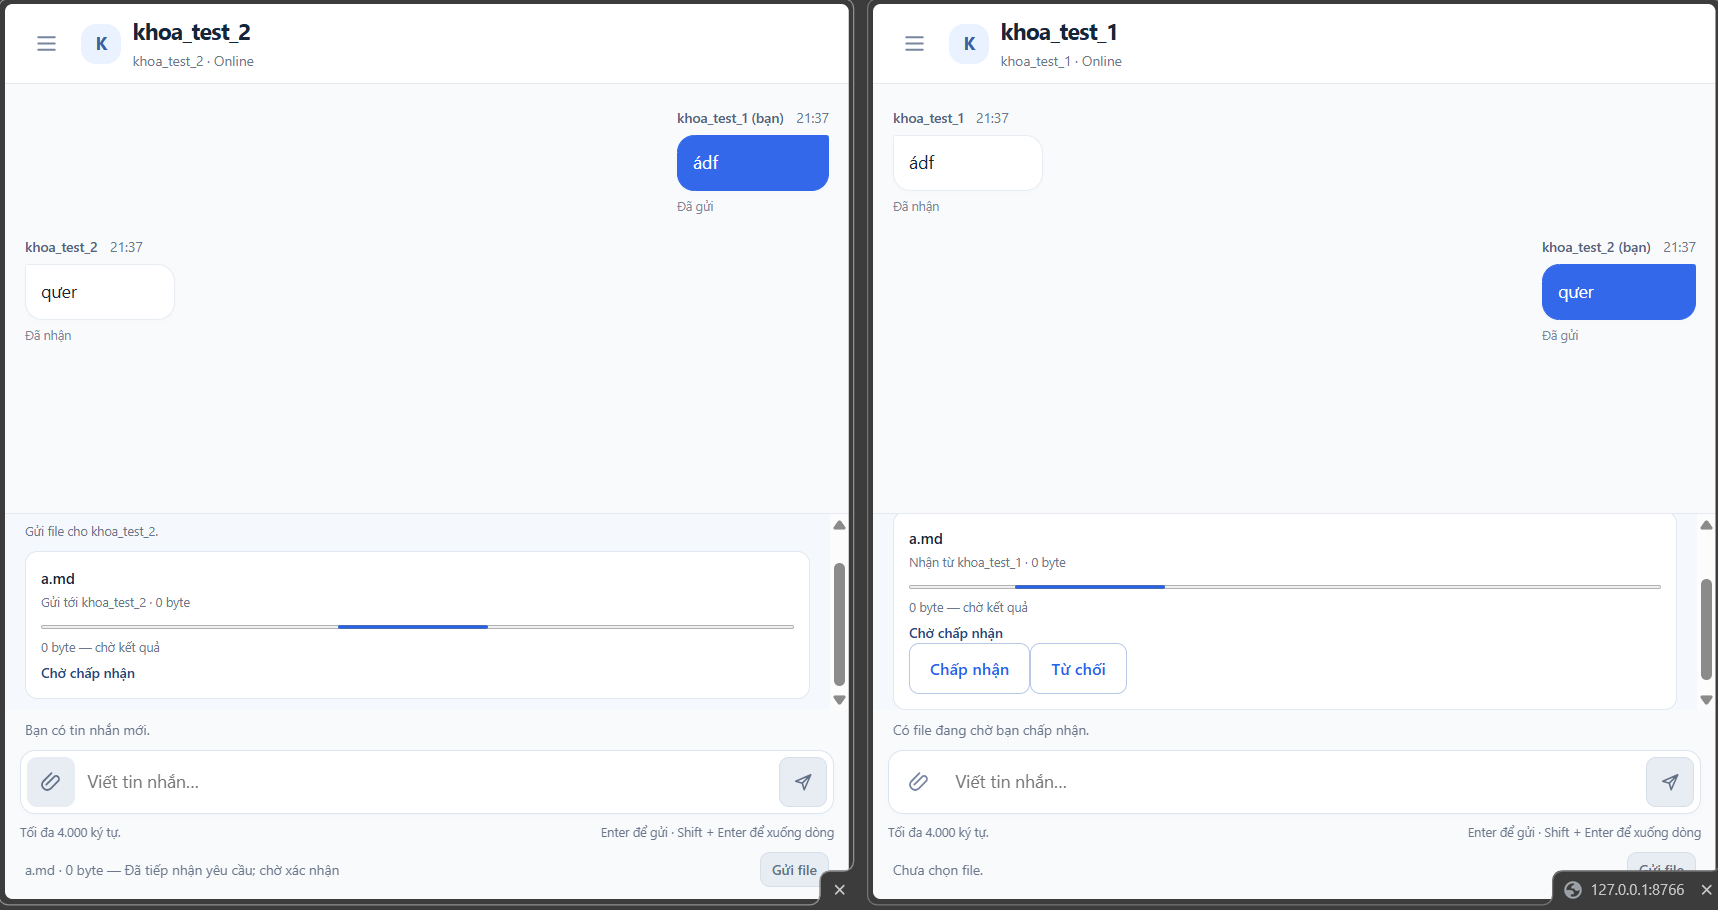
\includegraphics[width=\textwidth]{Assets/send_file.png}
    \caption{Chat riêng với thẻ file đang truyền và thanh tiến trình}
\end{figure}

\subsection{Khả năng truy cập và thích ứng thiết bị}
Trên máy tính, giao diện chia hai cột (thanh bên và khung chat), ô soạn tin luôn nằm trong vùng nhìn thấy và tự tăng chiều cao tới một giới hạn rồi cuộn bên trong. Trên điện thoại, danh sách cuộc trò chuyện thu thành ngăn kéo (drawer), có quản lý focus bằng bàn phím và đóng bằng phím Escape. Các thành phần tương tác có nhãn, trạng thái bằng chữ và focus rõ ràng. Danh sách thẻ file thu gọn được bằng bàn phím, và khi thu gọn vẫn hiển thị số lượt truyền đang chạy của cuộc trò chuyện đó.

\subsection{Giới hạn}
\begin{itemize}
    \item Phạm vi kiểm chứng là localhost trên Windows, chưa kiểm thử qua nhiều máy trong LAN.
    \item Kích thước file lớn nhất đã kiểm thử qua trình duyệt là 8MiB.
    \item Chưa có hộp thư gửi offline.
\end{itemize}